\documentclass[nofootinbib,amssymb,amsmath]{revtex4}
\usepackage{mathtools}
\usepackage{amsthm}
\usepackage{algorithm}
\usepackage{algpseudocode}
\usepackage{lmodern}
\usepackage{graphicx}
\usepackage{color}

%Put an averaged random variable between brackets
\newcommand{\ave}[1]{\left\langle #1 \right\rangle}
\newcommand{\HC}{\texttt{HaplotypeCaller}}
\newcommand{\Mutect}{\texttt{Mutect}}
\newcommand{\code}[1]{\texttt{#1}}
\newcommand{\mc}[1]{\mathcal{#1}}


\newtheorem{lemma}{Lemma}
\newtheorem{corollary}{Corollary}

\def\SL#1{{\color [rgb]{0,0,0.8} [SL: #1]}}
\def\DB#1{{\color [rgb]{0,0.8,0} [DB: #1]}}

\begin{document}

\title{Pair HMM probabilistic realignment in HaplotypeCaller and Mutect}
\author{David Benjamin\footnote{The author took no part in development of the methods described below -- credit belongs to several others on the GATK team. }}
\email{davidben@broadinstitute.org}
\affiliation{Broad Institute, 75 Ames Street, Cambridge, MA 02142}

\date{\today}

\begin{abstract}
After generating candidate haplotypes, the GATK tools \HC~and \Mutect~realign reads against these haplotypes to obtain a matrix of likelihoods for each read to be derived from each haplotype.  Here we describe the probabilistic model specifying this likelihood as well as its computational implementation.  We do not describe the translation of this implementation into native code optimized for vectorized architectures.
\end{abstract}

\maketitle

\section{The Pair HMM model}
We want to calculate the probability $P( \mc{R} | \mc{H})$ of read $\mc{R}$ to be sequenced from haplotype $\mc{H}$, where the haplotypes are sufficiently long that reads are contained within them.  This likelihood is the sum of likelihoods of all possible alignments $\mc{A}$ of $\mc{R}$ to $\mc{H}$:

\begin{equation}
P(\mc{R} | \mc{H}) = \sum_{\mc{A}} P(\mc{R}, \mc{A} | \mc{H})
\end{equation}

We represent alignments as sequences
\begin{equation}
{\rm alignment} = \{ (i_1, j_1, s_1), (i_2, j_2, s_2) \ldots (i_N, j_N, s_N) \},
\end{equation}
where $i$ and $j$ represent positions within the read and haplotype, respectively, and $s_n \in \{ M, I, D \}$ represents the states of match, insertion, and deletion of the read relative to the haplotype.  For example, an alignment $\{ (1,10, M), (2,11, M), (3,12, M), (4,13, M), (4,14, D), (4,15, D), (5,16, M), (6,17, M), (7,17, I), (8,18, M) \}$ means that positions 1 - 4 of the read match positions 10 - 13 of the haplotype, followed by a two-base deletion (advancing from 13 to 15 in the haplotype without advancing in the read), followed by a match of read positions 5 - 6 with haplotype positions 16 - 17, followed by an insertion at read position 7, followed by a match.  The allowable transitions $(i_n, j_n) \rightarrow (i_{n+1}, j_{n+1})$ are
\begin{itemize}
\item $(i, j, M/D/I) \rightarrow (i+1, j+1, M)$: match of read position $i+1$ with haplotype position $j + 1$
\item $(i, j, M/D) \rightarrow (i, j+1, D)$: deletion after read position $i$ -- haplotype position $j+1$ is deleted
\item $(i, j, M/I) \rightarrow (i + 1, j, I)$: insertion at read position $i + 1$
\end{itemize}
Note that the state label $s$ seems redundant because it can be reconstructed from the sequence of $i$ an $j$.  While this is true, our model treats indel starts differently from indel continuations, and by including the state label we can distinguish these conveniently\footnote{That is, we can tell which type of transition it is by looking back one unit instead of two.  Thus we have a first-order Markov model instead of a second-order Markov model.}.  These transitions are illustrated as a finite state machine in Figure \ref{fig:fsm}.

\begin{figure}
\center
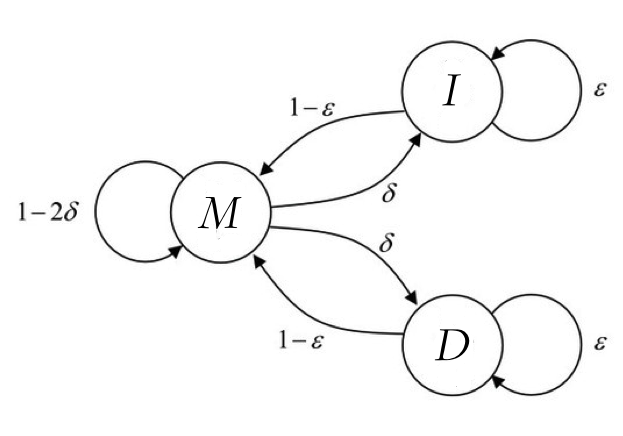
\includegraphics[scale=0.35]{finite_state.png}
\caption{Finite state machine of transitions among match, insertion, and deletion alignment states.  In the absence of per-base BQSR indel qualities transition probabilities are parametrized  by two constants, the indel start probability $\delta$ and the indel continuation probability $\epsilon$, such that $T_{MI} = T_{MD} = \delta$, $T_{MM} = 1 - 2 \delta$, $T_{II} = T_{DD} = \epsilon$, $T_{IM} = T_{DM} = 1 - \epsilon$, and $T_{ID} = T_{DI} = 0$.}
\label{fig:fsm}
\end{figure}

The read-alignment likelihood has two components.  First is the probability of the sequence of match, insertion, and deletion states, which is
\begin{equation}
P(\mc{A}) = \prod_k T_{s_k, s_{k+1}},
\end{equation}
where $T$ is a matrix of state transition probabilities\footnote{The gap continuation probability corresponds to a phred-scaled quality that is set by the \code{gcpHMM} argument, which is 10 by default, implying that $T_{DD} = T_{II} = 10^{-10/10} = 1/10$ and $T_{DM} = T_{IM} = 1 - T_{II}$.  The indel start transitions are derived from the read's BQSR base insertion and base deletion qualities, if they exist, or a phred-scaled indel start quality of 45 if they do not.  In production at the Broad Institute bams do not have BQSR indel qualities, hence the constant default is used.  That is, $T_{MD} = T_{MI} = 10^{-4.5}$ and $T_{MM} = 1 - 2 \times 10^{-4.5}$.}\footnote{The elements of $T$ are either empirical or, (sometimes) in the case of indel start transitions, derived from BQSR.  However in principle all elemnts of $T$ could be learned by applying the Baum-Welch algorithm to some known training data.  For example, one could use a haploid cell line, for which any assembly region has a single haplotype.}.  The index $k$ runs from 1 to the number of states in the alignment, that is, the read length plus the number of deleted reference bases.  Next is the emission probability of the read bases given the haplotype bases they align to and the base qualities:
\begin{equation}
P(\mc{R} | \mc{A}, \mc{H}) = \prod_k P(r_{i_k} | h_{j_k}, q_{i_k})^{{\rm I}[s_k = M]},
\end{equation}
where $r_m$ and $h_n$ are the $m$th read bases and $n$th haplotype base and $q_m$ is the quality of the read's $m$th base.  Note that this only includes alignments in the match state.  The per-base emission is given directly from the definition of base quality:
\begin{equation}
P(b_2 | b_1, q) = \left\{ \begin{array}{cc} \epsilon(q)/3 & (b_1 \ne b_2) \\ 1 - \epsilon(q) & (b_1 = b_2)  \end{array} \right.
\end{equation}
where $\epsilon(q) = 10^{-q/10}$ is the error rate implied by the phred-scaled quality $q$.

\section{Dynamic Programming}

Define the matrices $M$, $I$ and $D$ by $M_{ij} = $ the total likelihood of \textit{all} paths from the beginning of the read to position $i$ that end in a match state, and likewise for $D$ and $I$.  Then the recursions
\begin{align}
M_{ij} =& P(r_i | h_j, q_i) \left( M_{i-1,j-1} T_{MM} + I_{i-1,j-1} T_{IM} + D_{i-1,j-1} T_{DM} \right) \label{match} \\
I_{ij} =& M_{i-1,j} T_{MI} + I_{i-1,j} T_{II} \label{ins} \\
D_{ij} =& M_{i,j-1} T_{MD} + D_{i, j - 1} T_{DD} \label{del}
\end{align}
define the entire pair HMM algorithm:

\begin{algorithm}
\begin{algorithmic}[1]
\State Initialize $M_{0,j} = I_{0,j} = 0$ and $D_{0,j} = 2^{1020}/|\mc{H}|$ for $1 \le j \le |\mc{H}|$.
\For{$1 \le i \le | \mc{R} |$}
	\For{$1 \le j \le | \mc{H} |$}
		\State Calculate $M_{ij}$ via Equation \ref{match}.
		\State Calculate $I_{ij}$ via Equation \ref{ins}.
		\State Calculate $D_{ij}$ via Equation \ref{del}.
	\EndFor
\EndFor
\State Total likelihood $P(\mc{R} | \mc{H})$ is $\sum_j \left(M_{\mc{R},j} + I_{\mc{R},j} \right)$.
\end{algorithmic}
\caption{Pair HMM algorithm}
\label{pairHMM}
\end{algorithm}

That the $i = 0$ rows of $M$ and $I$ are initialized to zero corresponds to starting at an imaginary position one base before the read start in a deletion state\footnote{Since $T_{DI} = 0$ this means that an alignment may not start with an insertion, though it may begin with one.  This limitation is unnecessary and could be fixed by initializing the $i = 0$ row of $I$ to a non-zero value as well.}.  The factor of $1/|\mc{H}|$ corresponds to a flat prior on which $j$ an alignment starts at.  This is important for a local alignment because we don't want to penalize reads that start in the middle of the haplotype.  The curious factor of $2^{1020}$ is a huge number to prevent underflow -- all multiplications are by numbers less than 1, so we needn't worry about overflow -- which is a much more efficient approach than performing the computation in log space.  The omission of $D$ from the returned value recognizes the fact that a terminal deletion is meaningless.

Finally, we note a shortcut that the GATK exploits: when two consecutive haplotypes of the same length\footnote{The condition on the same length could easily be relaxed simply by accounting for the constant $1/|\mc{H}|$ initialization.}  agree up to the $k$th position, the first $k$ columns of $M$, $D$ and $I$ are recycled and the inner loop is over $k < j \le \mc{H}$.

\end{document}